\section{Inledning}

Systemet har utvecklats som en del av kursen TFYY51 under hösten 2019 av
studenter på Y-linjen.

\begin{figure}
	\centering
	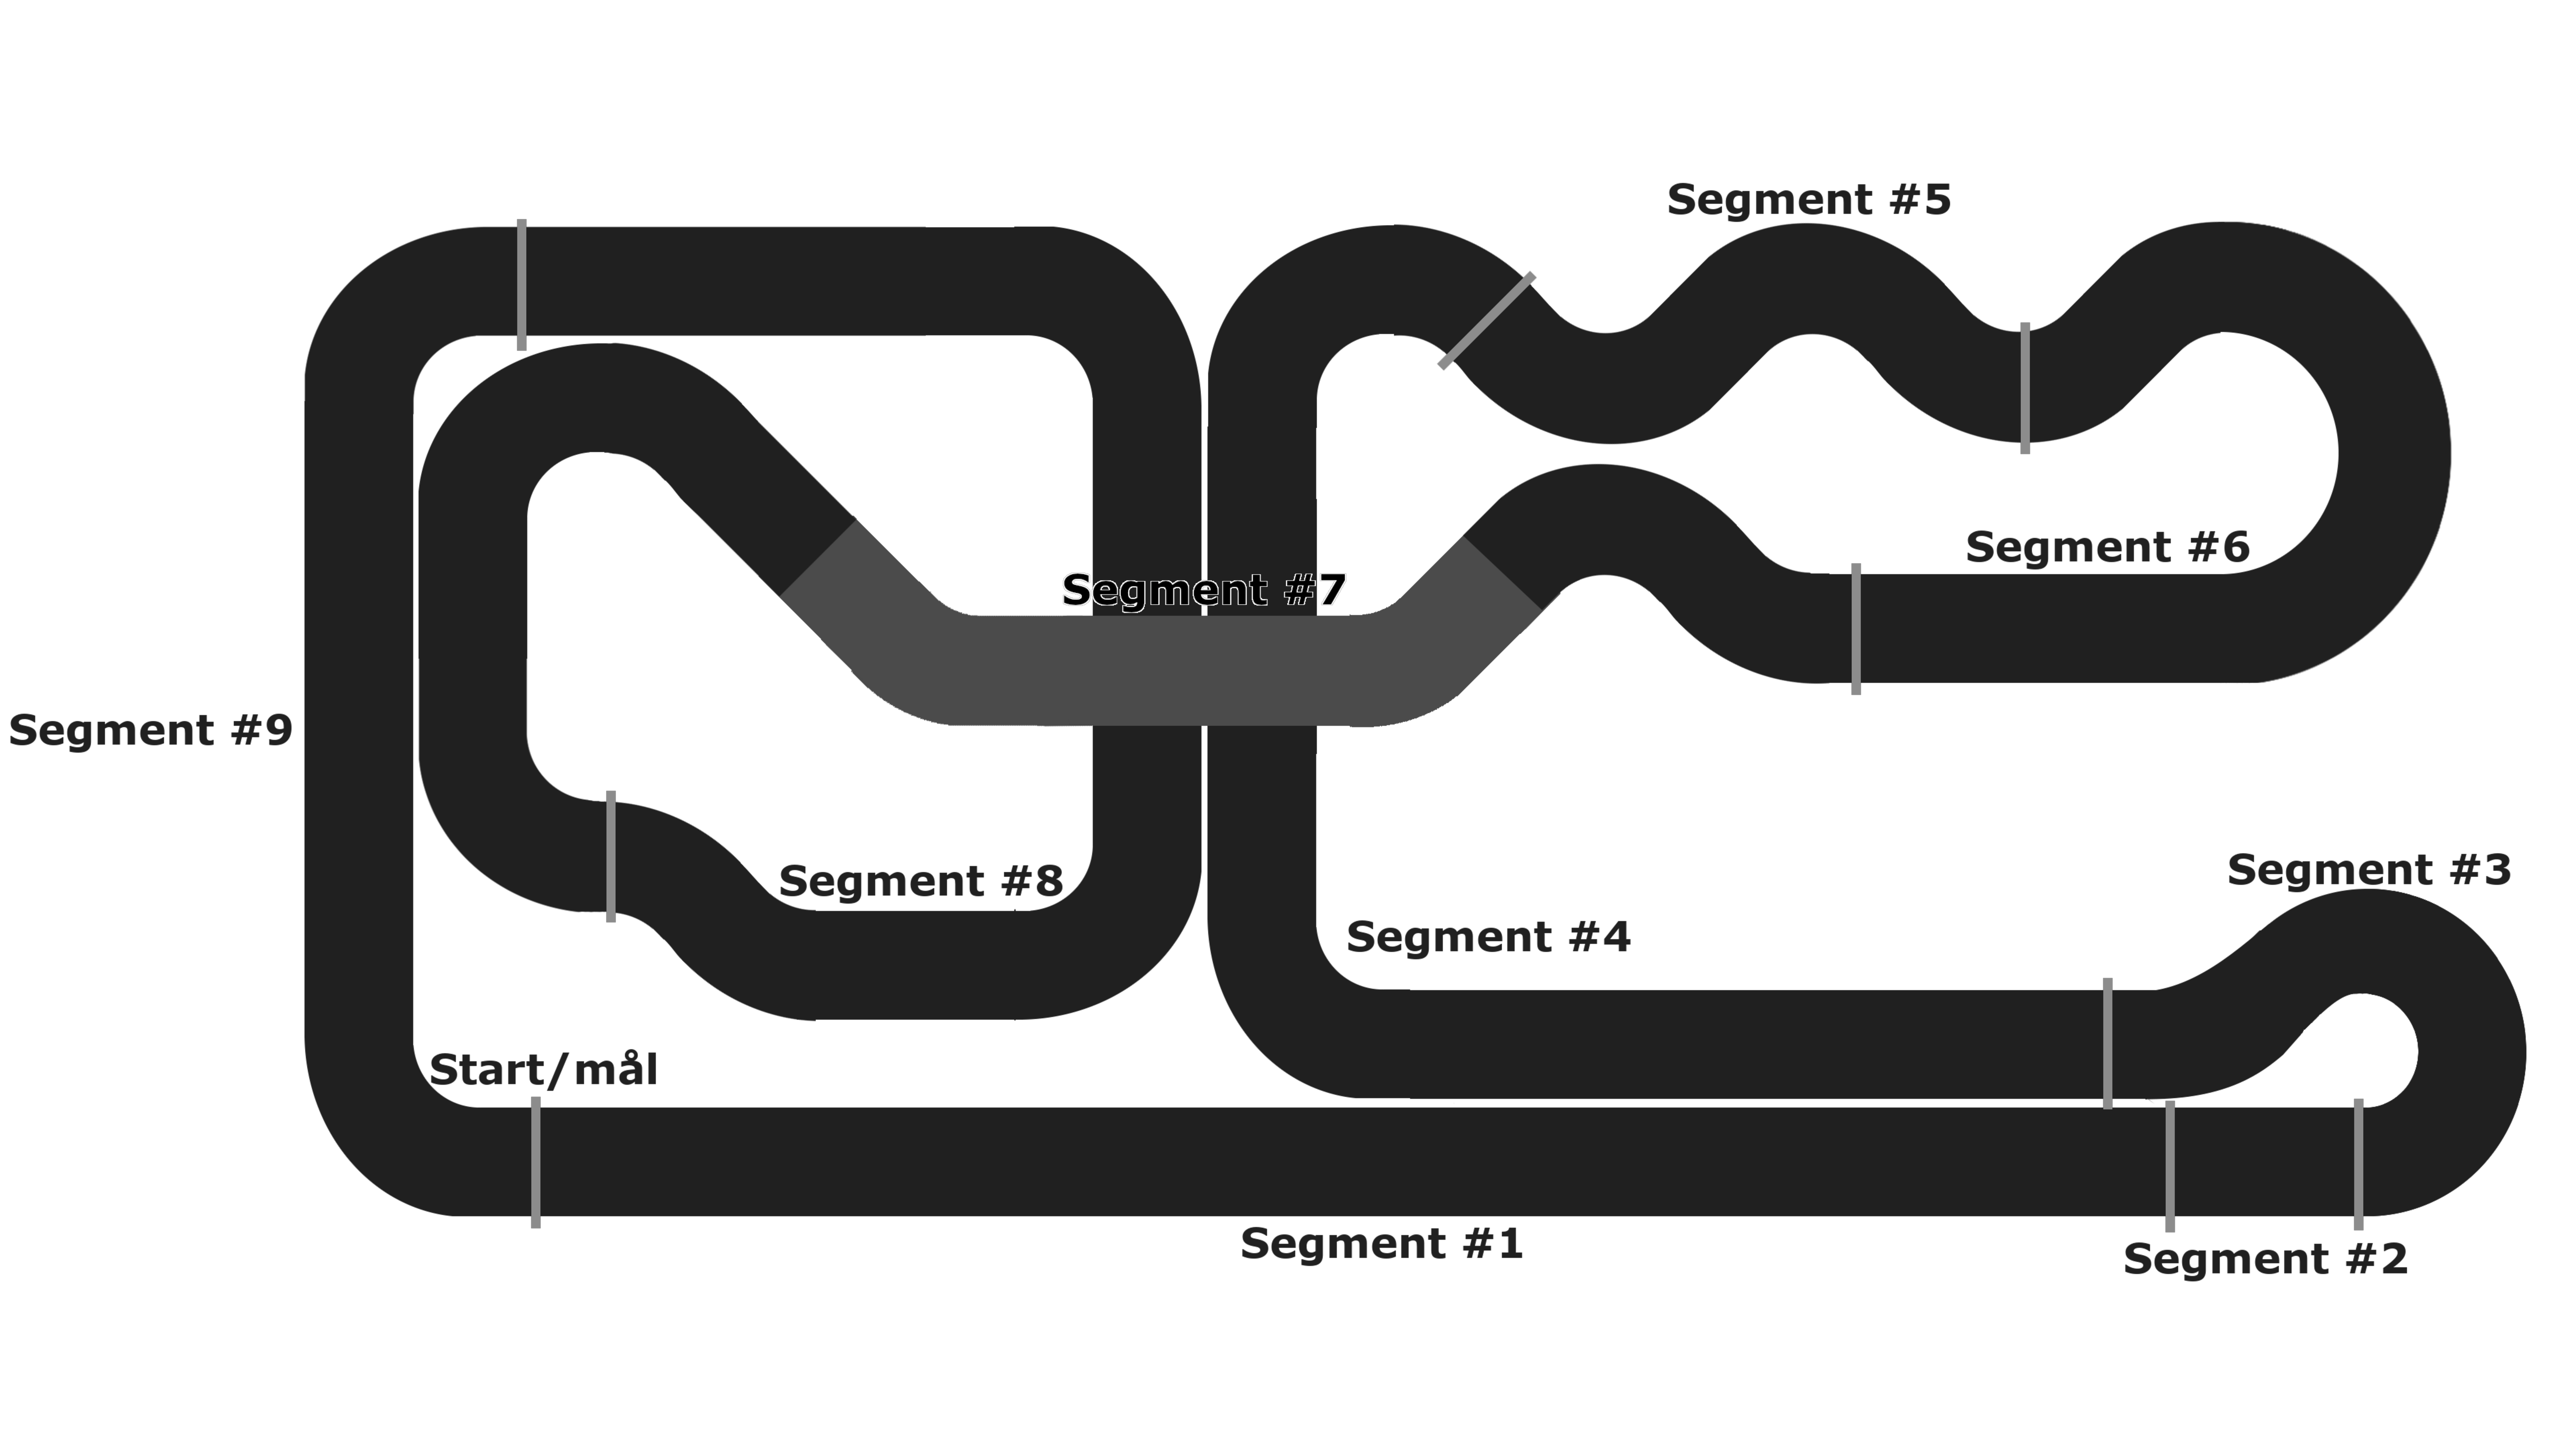
\includegraphics[width=\linewidth] {Figures/BanaModell}
	\caption{En modell av bilbanan.}
	\label{fig:bilbanan}
\end{figure} 

\subsection{Bakgrund} 

Projektet har utförts med hjälp av en bilbana samt flera bilar, givare,
spänningsaggregat och två datorer. Via en av datorerna har spänning tillförts
bilbanan. Med hjälp av givarna är det möjligt att veta när en bil är vid en viss
position. Programvaran har utvecklats i Matlab.

\subsection{Syfte och mål}

Syftet med projektet har varit att lära sig att arbeta utifrån
projektstyrningsmodellen LIPS. Målet med projektet var att konstruera ett system
som kan köra bilar runt en bilbana på en vald referenstid mellan 12 och 15
sekunder. Detta skulle göras för ett antal bilar med olika egenskaper. Fler krav
som skulle klaras av finns i kravspecifikationen. Se bilaga för
kravbeskrivningen och appendix~\ref{app:kravbeskrivning} för en beskrivning av
hur systemet klarade dessa krav.

